\chapter{Dokumentation af kode} \label{chap:kode_docs}
I dette kapitel vil funktioner i programmet blive forklaret.

\section{Loginsystem} \label{sec:login}
Formålet med et loginsystem er, at programmet kan holde styr på hvilken bruger der anvender systemet. 
Dette er vigtigt således reservationer placeres i det rigtige navn, og at brugeren kun har adgang til de rigtige funktioner. 
Eksempelvis skal et medlem af sejlklubben, ikke have adgang til at tilføje og fjerne brugere. 

Loginproceduren består fra brugeres synspunkt af at indtaste sit brugernavn og adgangskode, og trykke på login eller enter. 
Hvis brugeren har tastet rigtigt, vises deres en velkomstbesked og, afhængigt af brugerens privileger, får vedkommende adgang til de funktioner de har til rådighed.

Når loginkaldet udføres af brugeren, oprettes der en forbindelse til databasen, hvorefter den tjekker hvorvidt de informationer, som er givet, stemmer overens med dens. 
Dog anvendes der en kryptografisk hashing algoritme. Dette er for at undgå, at folk med adgang til databasen kan aflæse brugernes adgangskoder.
Det er en præventiv beskyttelse mod hacking angreb.
I programmet anvendes SHA-256, som returner en 256 bit hash (dvs. 32 bytes og 64 karakterer som en streng). 
Men dette ville være trivielt, at udskifte med en anden hashing algoritme, hvis der blev fundet en svaghed i SHA-256. 


\section{Klasser}
\subsection*{Medlemsklasse}
%Set imagepath and scaling, imagepath set to start in images/UmlMini folder, just write filename and extension
%FBox added for outline on items
\begin{wrapfigure}{l}{0.5\textwidth}
    \label{img:login_interface}
    \vspace{-20pt}
    \begin{center}
        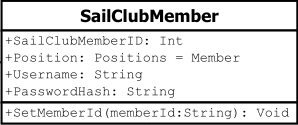
\includegraphics[width=0.48\textwidth]{UmlMini/SailClubMember.png}
    \end{center}
    \vspace{-20pt}
    \caption{SailClubMember}
    \vspace{-10pt}
\end{wrapfigure}
Basis medlemsklassen for systemet er SailClubMember. 
Klassen er en underklasse til den mere generelle Person klasse. 
Udbyggelsen i denne klasse er, at et medlem har et medlems Id, en position, et brugernavn og et password. 
Id'et bliver brugt i hele systemet til at identificere hvilken bruger der gør hvad. 

Positions feltet angiver at personen er et medlem i klubben. 
Positions feltet kan også sættes til at være administrator, i tilfælde at at personen er administrator. 
Positions feltet angiver desuden hvilke rettigheder de forskellige brugere har, fx har en administrator lov til at tilgå alle funktioner i programmet, mens et medlem ikke har lov til at gå ind i undervisnings delen af programmet. 

Brugernavn og password felterne anvendes i login systemet, som sikrer at hver bruger kan logge ind på systemet og sikre at de kan tilgå funktionerne.

SailClubMember klassen er central i programmet, da alle brugere/medlemmer af sejklubben skal oprettes som et SailClubMember og deri skal deres position i klubben angives, så de kan tilgå de funktioner i programmet som de kunne have gavn af. Derudover findes der i RegularSailTrip-klassen og Logbook-klassen referencer til SailClubMember. Dette gøres så at information om hvem der har foretaget en booking af en båd, og hvem der har skrevet logbogen til den sejltur der blev foretaget. Disse referencer er også vist på det fulde UML-diagram som findes i \myref{UML_diagram}
 
\subsection{Eventklasse}

\begin{wrapfigure}{l}{0.5\textwidth}
    \label{img:login_interface}
    \vspace{-20pt}
    \begin{center}
        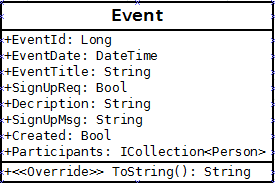
\includegraphics[width=0.48\textwidth]{UmlMini/Event.png}
    \end{center}
    \vspace{-20pt}
    \caption{Eventklasse}
    \vspace{-10pt}
\end{wrapfigure}
Eventklassen er den klasse om bruges til oprettelse af  begivenheder. Klassen består af 7 felter: EventDate, EventTitle, SignUpReq, Description, SignUpMsg, Created og så en liste af klassen Person, som hedder Participants.

Description er selve begivenhedsbeskrivelsen. 

Participantslisten bruges når folk skal tilmeldes til begivenhederne; hver begivenhed har sig egen liste med tilmeldte. 

Den eneste metode er en override af ToString, som retunerer Description.

